% !TEX root = ../agglo_clust_review.tex

\section{Introduction}
The majority of clustering methods work with positive edge weights only, representing for example attractive interactions between the nodes. These methods require the user to specify the desired numbers of clusters or a termination criterion (as in spectral clustering or iterated normalized cuts) or even a stronger version of supervision in terms of seeds (as in seeded watershed or random walker).  
Hierarchical clustering (HC) is also a popular method, which creates a hierarchy of clusters. Agglomerative HC is a bottom-up approach starting with each node assigned to its own cluster and incrementally merging clusters while moving up the hierarchy \cite{lance1967general}. This method usually requires the user to choose a level in the cluster hierarchy defining the desired output clustering. 

Other partitioning methods work with so-called \emph{signed graphs}, which include both positive and negative edge weights corresponding to attraction and repulsion between nodes. The advantage of using signed graphs is that balancing attraction and repulsion allows us to perform the clustering without defining additional parameters. This can be done optimally by solving the so-called \emph{multicut optimization problem} or \emph{correlation clustering} \cite{kappes2011globally,chopra1991multiway}. However, this problem is NP-hard, so heuristic approximated methods were proposed \cite{yarkony2012fast,pape2017solving}. For even larger problems, greedy agglomerative partitioning algorithms are usually employed \cite{kardoostsolving,keuper2015efficient}. Some of these approaches \cite{levinkov2017comparative,wolf2018mutex} also dynamically introduce cannot-link constraints, representing mutual exclusion relationships between clusters. Despite their similarity to agglomerative HC algorithms for unsigned graphs with only positive weights, neither an explicit connection nor a clear experimental comparison was proposed so far.

As a first contribution, we reformulate several of these recently proposed graph agglomerative algorithms in a simple review framework (Sec. \ref{sec:general_framework}) that represents a generalization of agglomerative HC to graphs with both attractive and repulsive edge weights (see Figure \ref{fig:intro_figure} for a visual abstract). From this new point of view, agglomerative HC and algorithms proposed in \cite{levinkov2017comparative,wolf2018mutex,lance1967general,kardoostsolving} all share a general procedure but differ in the way inter-cluster interaction is updated after each iteration (Table \ref{tab:linkage-criteria}). At the same time, we also show that this framework allows us to introduce totally new variations of these algorithms. 
Ultimately, by presenting this simple general approach, our hope is to motivate a deeper understanding of the connection between algorithms for unsigned and signed graphs.

We then evaluate and compare these algorithms on \emph{instance segmentation}, which is a computer vision task consisting in assigning each pixel of an image to an object instance. %, where the number of instances is usually not known in advance. 
For our experiments, we focus on a \emph{proposal-free} deep learning method that does not involve object detection but directly group pixels into object instances. Recently, there has been a growing interest for proposal-free methods, since in certain types of data, for example electron microscopy (EM) image volumes of neurons \cite{arganda2015crowdsourcing}, objects are not approximated well by bounding boxes.
We then use a CNN to predict the edge weights of a grid-graph such that each node represents a pixel of the image, similarly to \cite{liu2018affinity,lee2017superhuman,wolf2018mutex}, and provide these weights as input to the algorithms of our framework. 
By applying this method both to 2D urban scenes from the CityScapes dataset and a challenging neuron-segmentation task of 3D EM image stacks, we show how... \UPDATE{Summarize results}



% Most recently, success in instance segmentation (IS) has been achieved by applying deep learning and there are two main types of successful deep learning approaches to IS: proposal-based \cite{he2017mask,dai2016instance,li2017fully} and proposal-free \cite{kong2018recurrent,novotny2018semi,kulikov2018instance,kirillov2017instancecut} methods. Proposal-based methods consist of two steps: detecting objects, for example by finding bounding boxes, and assigning pixels to the detected instances. Although these approaches have proven to be highly successful in instance segmentation competitions like MS COCO \cite{lin2014microsoft}, Pascal VOC2012 \cite{everingham2010pascal} and CityScapes \cite{cordts2016cityscapes}, they are not applicable to certain types of data, for example electron microscopy (EM) image volumes of neurons \cite{arganda2015crowdsourcing}, where objects are not approximated well by bounding boxes. 
% More motivation: They are at the same time limited by the quality of the object detection routine, which is hard to train on small datasets (but no ref for this)
% Thus, there is a growing interest for more efficient proposal-free methods that perform IS by directly predicting \UPDATE{pixel features} and then grouping pixels into object instances. In this work, we focus on a common proposal-free method, where a Convolutional Neural Network (CNN) predicts affinities representing how likely it is for pairs of pixels to belong to the same instance. Recently, this approach was successfully applied both to neuron segmentation of 3D EM image stacks \cite{lee2017superhuman,wolf2018mutex} and instance segmentation of 2D urban scenes \cite{liu2018affinity}, where it achieved performances superior and comparable, respectively, to proposal-based methods.
% In this approach, the output of the CNN can be represented as a weighted grid graph such that each node represents a pixel of the image and the weights of the edges define interactions between the pixels. A graph clustering algorithm is then applied to cluster pixels into instances. 
% Finally, the algorithms included in the framework are evaluated on an instance segmentation task, both on 3D biological image stacks (Sec. \ref{sec:neuro_segm_exp}) and 2D urban scenes (Sec. \ref{sec:cityscapes_exp}). Our analysis highlights strengths and weaknesses of each algorithm by comparing their robustness to noise, efficiency and inclination to output a well balanced graph partitioning.



\begin{figure}[t]
\centering
% 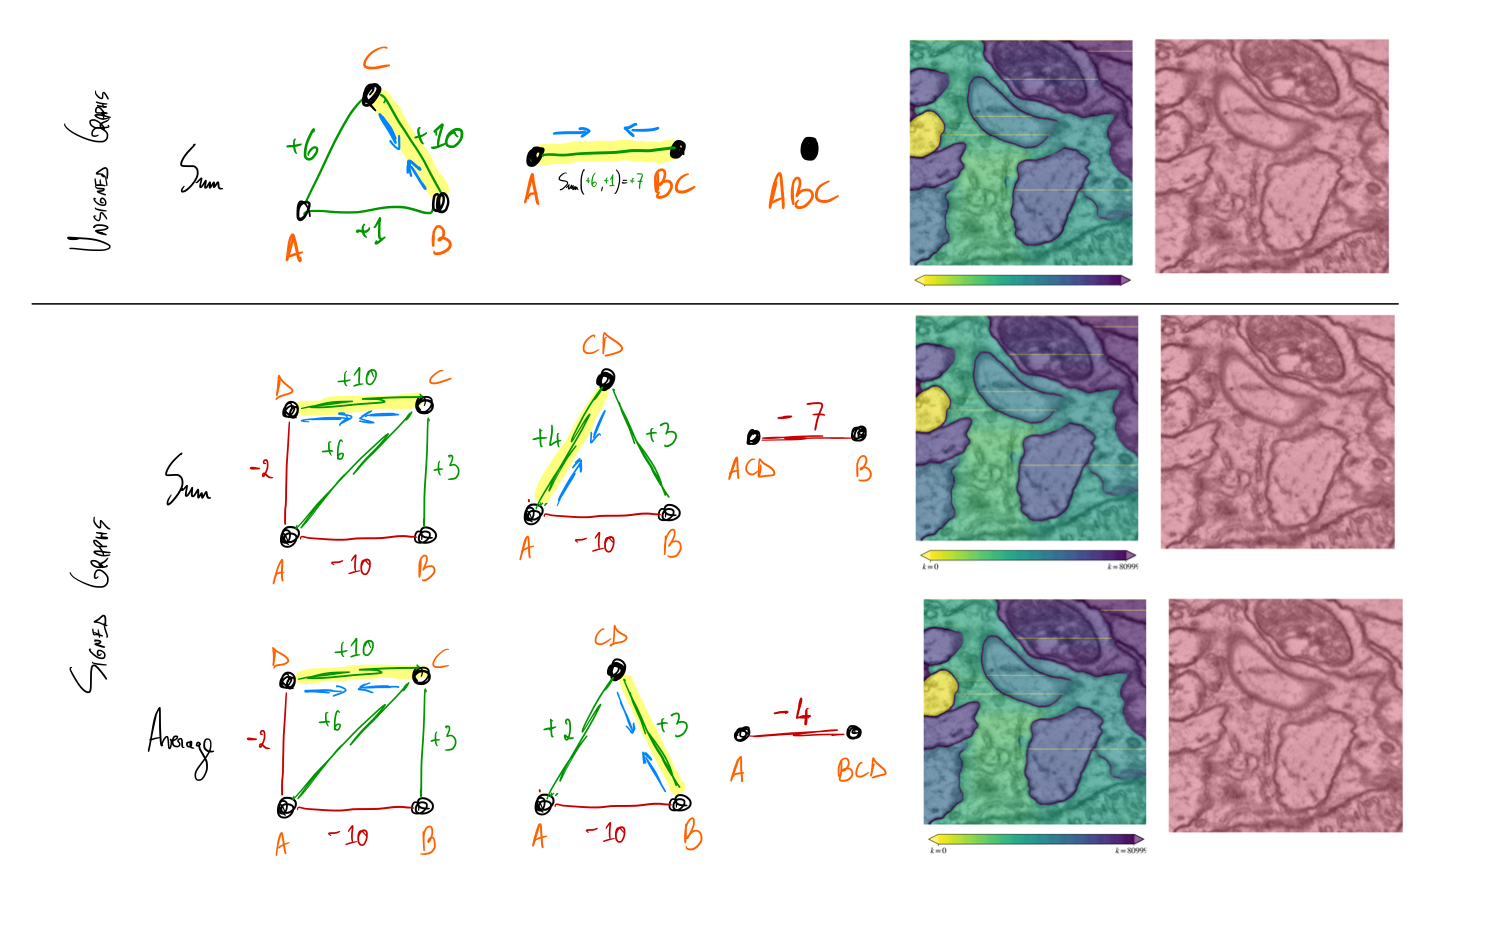
\includegraphics[width=0.5\textwidth,trim=0.4in 1.2in 0.in 0.05in,clip]{./figs/intro_image.jpg} % left bottom right top
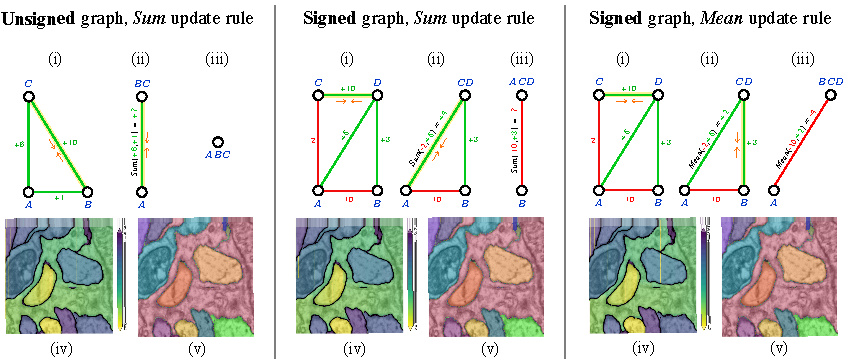
\includegraphics[width=\textwidth]{./figs/intro_image.pdf} % left bottom right top
\caption{
 (\textbf{a}) Some iterations of the generalized algorithm on toy graphs with attractive (green) and repulsive (red) interactions. (\textbf{b}) Example of CREMI 2016 neuron-segmentation data \cite{cremiChallenge} overlaid with instance segmentation. (\textbf{c}) Agglomeration order, representing which pairs of neighboring pixels were merged first (white), later on (brown) or never (black).
We note how similar linkage criteria, like \emph{Sum} (in the middle) and \emph{Average} (on the right), lead to strongly different merging orders. 
% On the left: a single cluster is returned with only attractive interactions.
 % main ideas and contributions
\label{fig:intro_figure}}
\end{figure}
